\chapter{Mobile Transport Layer}

Supporting mobility only on lower layers up to the network layer is not enough to provide mobility support for applications. Most applications rely on a transport layer, such as \gls{tcp} or \gls{udp} in the case of the Internet. 

Two functions of the transport layer in the internet are: 
\begin{itemize}
	\item checksumming over user data and 
	\item multiplexing/demultiplexing of data from/to applications.
\end{itemize}

%While the network layer only addresses a host, ports in \gls{udp} or \gls{tcp} allow dedicated applications to be addressed. The connection-less UDP does not offer much more than this addressing, so, the following concentrates on TCP. While UDP is connection-less and
%does not give certain guarantees about reliable data delivery, TCP is much more
%complex and, needs special mechanisms to be useful in mobile environments.
%Mobility support in IP (such as mobile IP) is already enough for UDP to work.
%
%The main difference between UDP and TCP is that TCP offers connections
%between two applications. Within a connection TCP can give certain guarantees, such as in-order delivery or reliable data transmission using retransmission
%techniques. TCP has built-in mechanisms to behave in a ‘network friendly’
%manner. If, for example, TCP encounters packet loss, it assumes network internal congestion and slows down the transmission rate. This is one of the main
%reasons to stay with protocols like TCP. One key requirement for new develop-
%ments in the internet is ‘TCP friendliness'. UDP requires that applications
%handle reliability, in order delivery etc. UDP does not behave in a network
%friendly manner, i.e., does not pull back in case of congestion and continues to
%send packets into an already congested network.


\section{Traditional TCP}
Several mechanisms of the \gls{tcp} that influence the efficiency of \gls{tcp} in a mobile environment are:

\subsection{Congestion Control}

\begin{itemize}
	\item TCP has been designed for fixed networks with fixed end-systems.
	\item Data transmission takes place using network adapters, fiber optics, copper wires, special hardware for routers etc.
	\item Most of the hardware/software is not responsible for lost packets or bits flipping.
	\item The probable reason for a packet loss in a fixed network is a \textit{state of congestion at a node}.
	\item Router drops packets when the packet buffers of a router are filled and router cannot forward the packets fast enough because sum of input rates of packets destined is higher than the capacity of the output.
	\item A dropped packet is lost for the transmission, and the receiver notices a gap in the packet stream.
	\item Receiver does not tell sender if packet is missing, bit continues to acknowledge packets in sequence up to the missing one.
	\item When sender notices missing acknowledgment, it assumes a packet loss due to congestion and re-transmits the missing packet at full speed. This increases congestion.
	\item To mitigate congestion, \gls{tcp} slows down the transmission rate dramatically. 
\end{itemize}

\subsection{Slow Start}
The behavior \gls{tcp} shows after the detection of congestion is called \textit{slow start}.

\begin{itemize}
	\item The sender always calculates a congestion window for a receiver. 
	\item The start size of the congestion window is one segment (\gls{tcp} packet). 
	\item The sender sends one packet and waits for acknowledgment. 
	\item If this acknowledgment arrives, the sender increases the congestion window by one, now sending two packets (congestion window = 2). 
	\item This scheme doubles the congestion window every time the acknowledgments come back, which
	takes \gls{rtt}. 
	\item This is called the exponential growth of the congestion window in the slow start mechanism.
\end{itemize}


The exponential growth stops at the congestion \textit{threshold}. As soon as the congestion window reaches the congestion threshold, further increase of the transmission rate is only linear by adding 1 to the congestion window each time the acknowledgments come back.

Linear increase continues until a time-out at the sender occurs due to a missing acknowledgment, or until the sender detects a gap in transmitted data because of continuous acknowledgments for the same packet. In either case the sender sets the congestion threshold to half of the current congestion window.

%The congestion window itself is set to one segment and the sender starts sending
%a single segment. The exponential growth (as described above) starts once more
%up to the new congestion threshold, then the window grows in linear fashion.


\subsection{Fast Re-transmit/Fast Recovery}
Two things lead to a reduction of the congestion threshold:

\begin{itemize}
	\item One is a sender receiving continuous acknowledgments for the same packet. 
	\begin{itemize}
		\item This informs the sender of two things. One is that the receiver got all packets up to the acknowledged packet in sequence. In TCP, a receiver sends acknowledgments only if it receives any packets from the sender. Receiving acknowledgments from a
		receiver also shows that the receiver continuously receives something from the sender. The gap in the packet stream is not due to severe congestion, but a
		simple packet loss due to a transmission error. The sender can now re-transmit the missing packet(s) before the timer expires. This behavior is called \textit{fast re-transmit}.
		
		\item The receipt of acknowledgments shows that there is no congestion to justify a slow start. The sender can continue with the current congestion window. The sender performs a fast recovery from the packet loss.
	\end{itemize}
	

	\item The other reason for activating slow start is a time-out due to a missing acknowledgment.
\end{itemize} 



\subsection{Implications on Mobility}

\begin{itemize}
	\item \textit{Slow start} decreases the efficiency of \gls{tcp} if used together with mobile receivers
	or senders. The reason being the use slow start under the wrong assumptions.
%	\item From a missing acknowledgment, \gls{tcp} concludes a congestion situation.
	\item Error rates on wireless links are orders of magnitude higher compared to fixed fiber or copper links.
	\item Mobility can cause packet loss. There are many situations where a soft
	handover from one access point to another is not possible for a mobile end system. 
	\item Standard TCP reacts with slow start if acknowledgments are missing, which does not help in the case of transmission errors over wireless links and which does not really help during handover. This behavior results in a severe performance degradation of an unchanged \gls{tcp} if used together with wireless links or mobile nodes.
\end{itemize}

\section{Classical TCP Improvements}
Together with the introduction of \gls{wlan}s in the mid-nineties several research projects were started with the goal to increase \gls{tcp}’s performance in wireless and mobile environments.

\subsection{Indirect TCP (I-TCP)}
Two competing insights led to the development of {I-TCP}:
\begin{itemize}
	\item \gls{tcp} performs poorly together with wireless links.
	\item \gls{tcp} within the fixed network cannot be changed.
\end{itemize}

I-TCP segments a \gls{tcp} connection into:
\begin{multicols}{2}
	\begin{enumerate}[label=\alph*)]
		\item a fixed part and
		\item a wireless part.
	\end{enumerate}
\end{multicols}


Figure \ref{fig:indirect_tcp} shows an example with a mobile host connected via a wireless link and an access point to the ‘wired’ internet where the correspondent host resides. The correspondent node could also use wireless access. 
\begin{itemize}
	\item Standard TCP is used between the fixed computer and the access point. No computer in the internet recognizes any changes to \gls{tcp}. 
	\item Instead of the mobile host, the access point now terminates the standard \gls{tcp} connection, acting as a proxy. 
	\item This means that the access point is now seen as the mobile host for the fixed host and as the fixed host for the mobile host. 
	\item Between the access point and the mobile host, a special \gls{tcp}, adapted to wireless links, is used. 
	\item A good place for segmenting the connection between mobile host and correspondent host is at the foreign agent of mobile IP. 
	\item The foreign agent controls the mobility of the mobile host anyway and can also hand over the connection to the next foreign agent when the mobile host moves on. 
\end{itemize}



%%%%%%%%%%%%%%%%%%%%%%%%%%%%%%%%%%%%%
%									%
%			FIGURE					%
%									%
%%%%%%%%%%%%%%%%%%%%%%%%%%%%%%%%%%%%%

\begin{figure}[ht!]
	\centering
	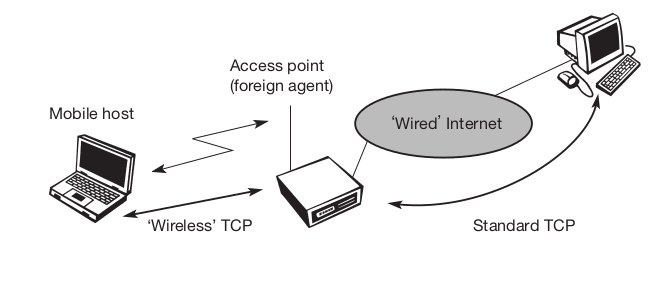
\includegraphics[width=0.8\textwidth]{indirect-tcp}
	\caption{Indirect TCP segments a TCP connection into two parts}\label{fig:indirect_tcp}
\end{figure}


The correspondent host in the fixed network does not notice the wireless link or the segmentation of the connection. The foreign agent acts as a proxy and relays all data in both directions. If the correspondent host sends a packet, the foreign agent acknowledges this packet and tries to forward the packet to the mobile host. If the mobile host receives the packet, it acknowledges the packet. However, this acknowledgment is only used by the foreign agent. If a packet is lost on the wireless link due to a transmission error, the correspondent host would not notice this. In this case, the foreign agent tries to re-transmit this packet locally to maintain reliable data transport.

Similarly, if the mobile host sends a packet, the foreign agent acknowledges this packet and tries to forward it to the correspondent host. If the packet is lost on the wireless link, the mobile hosts notice this much faster due to the lower round trip time and can directly re-transmit the packet. Packet loss in the wired network is now handled by the foreign agent.


\begin{itemize}
	\item I-TCP requires several actions as soon as a handover takes place (see Figure \ref{fig:socket-state-migration}). 
	\item In the example shown, the access point acts as a proxy buffering packets for re-transmission. 
	\item After the handover, the old proxy must forward buffered data to the new proxy because it has already acknowledged the data. 
	\item After registration with the new foreign agent, this new foreign agent can inform the old one about its location to enable packet forwarding. 
	\item Besides buffer content, the sockets of the proxy, too, must migrate to the new foreign agent located in the access point. 
	\item The socket reflects the current state of the \gls{tcp} connection, i.\ e.\, sequence number, addresses, ports etc. No new connection may be
	established for the mobile host, and the correspondent host must not see any changes in connection state.
\end{itemize}


%%%%%%%%%%%%%%%%%%%%%%%%%%%%%%%%%%%%%
%									%
%			FIGURE					%
%									%
%%%%%%%%%%%%%%%%%%%%%%%%%%%%%%%%%%%%%

\begin{figure}[hb!]
	\centering
	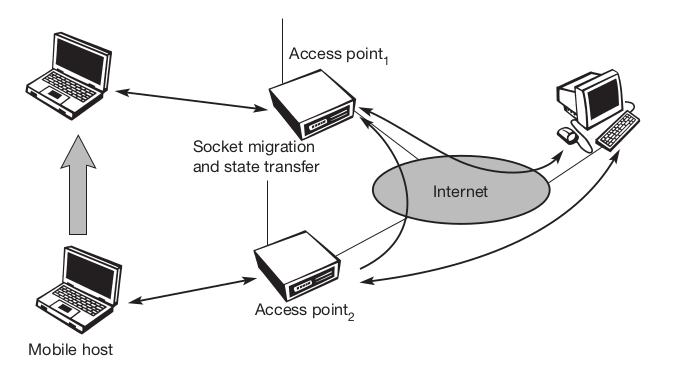
\includegraphics[width=0.8\textwidth]{socket-and-state-migration}
	\caption{Socket and state migration after handover of a mobile host}\label{fig:socket-state-migration}
\end{figure}

\subsubsection[Advantages]{Advantages With I-TCP}
There are several advantages with I-TCP:

\begin{itemize}
	\item I-TCP does not require any changes in the \gls{tcp} protocol.
	\item All current optimizations for \gls{tcp} still work between the foreign agent and the corresponding host.
	
	\item Due to the strict partitioning into two connections, transmission errors on the wireless link, i.\ e.\ , lost packets, cannot propagate into the fixed network.

    \item Introduction to new mechanism into a huge network is always dangerous. I-TCP ensures Different solutions can be tested or used at the same time without jeopardizing the stability of the network.
    
    \item Optimizing new mechanism is simple because they only cover one single hop.
    
	\item An optimized \gls{tcp} could use precise timeouts to guarantee retransmission as fast as possible. 
	
	\item Partitioning into two connections also allows the use of a different transport layer protocol between the foreign agent and the mobile host.
	
\end{itemize}

\subsubsection[Disadvantages]{I-TCP Disadvantages}
Idea of segmentation in I-TCP also comes with some disadvantages:

\paragraph*{Loss of End-to-End Semantics}
 The loss of the end-to-end semantics of \gls{tcp} might cause problems if the foreign agent partitioning the \gls{tcp} connection crashes.
 
 \paragraph*{Handover Latency}
 Increased handover latency may be much more problematic. All packets sent by the correspondent host are buffered by the foreign
 agent besides forwarding them to the mobile host.
 
 \paragraph*{Security Mechanism}
 The foreign agent must be a trusted entity because the \gls{tcp} connections
 end at this point. If users apply end-to-end encryption, e.\ g.\, the foreign agent has to be integrated into all security mechanisms.
 

\subsection{Snooping TCP}
One of the drawbacks of I-TCP is the segmentation of the single \gls{tcp} connection into two \gls{tcp} connections. This loses the original end-to-end \gls{tcp} semantic. The following \gls{tcp} enhancement works completely transparently and leaves the \gls{tcp} end-to-end connection intact.

The main function of the enhancement is to buffer data close to the mobile host to perform fast local re-transmission in case of packet loss.

\begin{itemize}
	\item In this approach, the foreign agent buffers all packets with destination
	mobile host and additionally \textit{snoops} the packet flow in both directions to recognize acknowledgments.
	\item The reason for buffering packets toward the mobile node is to enable the foreign agent to perform a local re-transmission in case of packet loss on the wireless link. 
	\item The foreign agent buffers every packet until it receives an acknowledgment from the mobile host.
	\item If the foreign agent does not receive an acknowledgment from the mobile host within a certain amount of time, either the packet or the acknowledgment has been lost.
	\item Alternatively, the foreign agent could receive a duplicate ACK which also shows the loss of a packet.
	\item Now the foreign agent re-transmits the packet directly from the buffer, performing a much faster re-transmission compared to the correspondent host. 
	\item The time out for acknowledgments can be much shorter, because it reflects only the delay of one hop plus processing time.
	
\end{itemize}


%%%%%%%%%%%%%%%%%%%%%%%%%%%%%
%							%
%		FIGURE				%
%							%
%%%%%%%%%%%%%%%%%%%%%%%%%%%%%

\begin{figure}[ht!]
	\centering
	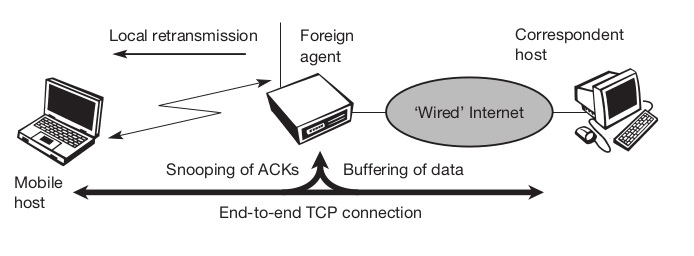
\includegraphics[width=0.9\textwidth]{snooping-tcp}
	\caption{Snooping TCP as a transparent TCP extension}\label{fig:snooping-tcp}
\end{figure}


%To remain transparent, the foreign agent must not acknowledge data to the correspondent host. This would make the correspondent host believe that the mobile host had received the data and would violate the end-to-end semantic in case of a foreign agent failure. However, the foreign agent can filter the duplicate acknowledgments to avoid unnecessary re-transmissions of data from the correspondent host. If the foreign agent now crashes, the time-out of the correspondent host still works and triggers a re-transmission. The foreign agent may discard duplicates of packets already re-transmitted locally and acknowledged by the mobile host. This avoids unnecessary traffic on the wireless link.

Data transfer from the mobile host with destination correspondent host works as follows. 
\begin{itemize}
	\item The foreign agent snoops into the packet stream to detect gaps in the sequence numbers of TCP.
	\item As soon as the foreign agent detects a missing packet, it returns a negative acknowledgment (NACK) to the mobile host. 
	\item The mobile host can now re-transmit the missing packet immediately. 
	\item Reordering of packets is done automatically at the correspondent host by TCP.
	
\end{itemize}


\subsubsection[Advantages]{Advantages of Snooping TCP}
Extending the functions of a foreign agent with a \textit{snooping TCP} has several advantages:

\paragraph*{Preserve End-to-End Semantics}
The end-to-end TCP semantic is preserved. No matter at what time the foreign agent crashes, neither the correspondent host nor the mobile host have an
inconsistent view of the TCP connection as is possible with I-TCP. The approach automatically falls back to standard TCP if the enhancements
stop working.

\paragraph*{Change in Correspondent Host Not Required}
The correspondent host does not need to be changed; most of the enhancements are in the foreign agent. Supporting only the packet stream from the
correspondent host to the mobile host does not even require changes in the mobile host.

\paragraph*{Immediate Handover of State Not Required}
It does not need a handover of state as soon as the mobile host moves to another foreign agent. Assume there might still be data in the buffer not
transferred to the next foreign agent. All that happens is a time-out at the correspondent host and re-transmission of the packets, possibly already to
the new care-of address.

\paragraph*{Automatic Fallback to Standard Solution}
It does not matter if the next foreign agent uses the enhancement or not. If not, the approach automatically falls back to the standard solution. This is one of the problems of I-TCP.

%\begin{itemize}
%	\item The end-to-end TCP semantic is preserved. No matter at what time the foreign agent crashes (if this is the location of the buffering and snooping
%	mechanisms), neither the correspondent host nor the mobile host have an
%	inconsistent view of the TCP connection as is possible with I-TCP. The
%	approach automatically falls back to standard TCP if the enhancements
%	stop working.
%	
%	\item The correspondent host does not need to be changed; most of the enhancements are in the foreign agent. Supporting only the packet stream from the
%	correspondent host to the mobile host does not even require changes in the
%	mobile host.
%	
%	\item It does not need a handover of state as soon as the mobile host moves to
%	another foreign agent. Assume there might still be data in the buffer not
%	transferred to the next foreign agent. All that happens is a time-out at the
%	correspondent host and re-transmission of the packets, possibly already to
%	the new care-of address.
%	
%	\item It does not matter if the next foreign agent uses the enhancement or not. If
%	not, the approach automatically falls back to the standard solution. This is
%	one of the problems of I-TCP, since the old foreign agent may have already
%	signaled the correct receipt of data via acknowledgements to the correspondent host and now has to transfer these packets to the mobile host via the
%	new foreign agent.
%\end{itemize}

\subsubsection[Disadvantages]{Disadvantages of Snooping TCP}
The simplicity of the scheme also results in some disadvantages:

\paragraph*{No Proper Wireless Link Isolation}
Snooping TCP does not isolate the behavior of the wireless link as well as I-TCP. The quality of the isolation, which snooping TCP offers, strongly depends on the quality of the wireless link, time-out values, and further traffic characteristics. It is problematic that the wireless link exhibits very high delays compared to the wired link due to error correction.


\paragraph*{Lack of Transparency}
Using negative acknowledgments between the foreign agent and the mobile host assumes additional mechanisms on the mobile host. This approach is no longer transparent for arbitrary mobile hosts.

\paragraph*{Incompatible With Encryption}
All efforts for snooping and buffering data may be useless if certain encryption schemes are applied end-to-end between the correspondent host and
mobile host. 


%\begin{itemize}
%	\item Snooping TCP does not isolate the behavior of the wireless link as well as I-TCP. Assume, for example, that it takes some time until the foreign agent
%	can successfully retransmit a packet from its buffer due to problems on the
%	wireless link (congestion, interference). Although the time-out in the foreign agent may be much shorter than the one of the correspondent host,
%	after a while the time-out in the correspondent host triggers a retransmission. The problems on the wireless link are now also visible for the correspondent host and not fully isolated. The quality of the isolation, which
%	snooping TCP offers, strongly depends on the quality of the wireless link,
%	time-out values, and further traffic characteristics. It is problematic that the
%	wireless link exhibits very high delays compared to the wired link due to
%	error correction on layer 2 (factor 10 and more higher). This is similar to I-TCP. If this is the case, the timers in the foreign agent and the
%	correspondent host are almost equal and the approach is almost ineffective.
%	
%	
%	\item Using negative acknowledgments between the foreign agent and the
%	mobile host assumes additional mechanisms on the mobile host. This
%	approach is no longer transparent for arbitrary mobile hosts.
%	
%	\item All efforts for snooping and buffering data may be useless if certain encryption schemes are applied end-to-end between the correspondent host and
%	mobile host. Using IP encapsulation security payload the TCP protocol header will be encrypted – snooping on the
%	sequence numbers will no longer work. Retransmitting data from the foreign agent may not work because many security schemes prevent replay
%	attacks – retransmitting data from the foreign agent may be misinterpreted
%	as replay. Encrypting end-to-end is the way many applications work so it is
%	not clear how this scheme could be used in the future. If encryption is used
%	above the transport layer (e.g., SSL/TLS) snooping TCP can be used.
%\end{itemize}


\subsection{Mobile TCP}

Dropping packets due to a handover or higher bit error rates is not the only phenomenon of wireless links and mobility — the occurrence of lengthy and/or frequent disconnections is another problem. Quite often mobile users cannot connect at all. 


%A TCP sender tries to re-transmit data controlled by a re-transmission timer that doubles with each unsuccessful re-transmission attempt, up to a maximum of one minute (the initial value depends on the round trip time). This means that the sender tries to retransmit an unacknowledged packet every minute and will give up after 12 retransmissions. What happens if connectivity is back earlier than this? No data is successfully transmitted for a period of one minute! The retransmission time-out is still valid and the sender has to wait. The sender also goes into slow-start because it assumes congestion.

%What happens in the case of I-TCP if the mobile is disconnected? The proxy has to buffer more and more data, so the longer the period of disconnection, the more buffer is needed. If a handover follows the disconnection, which is typical, even more state has to be transferred to the new proxy. The snooping approach also suffers from being disconnected. The mobile will not be able to send ACKs so, snooping cannot help in this situation.

The \textbf{M-TCP (mobile TCP)}\footnote{Mobile TCP does not have the same status as mobile IP, which is an internet RFC.} approach has the same goals as I-TCP and snooping TCP: 
\begin{itemize}
	\item to prevent the sender window from shrinking if bit errors or disconnection but not congestion cause current problems.
\end{itemize}

M-TCP wants to improve overall throughput:

\begin{itemize}
	\item to lower the delay, 
	\item to maintain end-to-end semantics of TCP, and 
	\item to provide a more efficient handover. 
\end{itemize}


Additionally, M-TCP is especially adapted to the problems arising from lengthy or frequent disconnections.

M-TCP splits the TCP connection into two parts as I-TCP does. 
\begin{itemize}
	\item An unmodified TCP is used on the standard host-supervisory host (SH) connection, 
	\item while an optimized TCP is used on the SH-MH connection.
\end{itemize}


The supervisory host is responsible for exchanging data between both parts similar to the proxy in I-TCP (see Figure \ref{fig:indirect_tcp}). The M-TCP approach assumes a relatively low bit error rate on the wireless link. Therefore, it does not perform caching/re-transmission of data via the SH. If a packet is lost on the wireless link, it has to be re-transmitted by the original sender. This maintains the TCP end-to-end semantics.

\begin{itemize}
	\item The SH monitors all packets sent to the MH and ACKs returned from the MH. 
	\item If the SH does not receive an ACK for some time, it assumes that the MH is disconnected. It then chokes the sender by setting the sender’s window size to 0.
	\item Setting the window size to 0 forces the sender to go into \textit{persistent mode}, i.\ e.\ ,
	the state of the sender will not change no matter how long the receiver is disconnected. This means that the sender will not try to retransmit data. 
	\item As soon as the SH (either the old SH or a new SH) detects connectivity again, it reopens the window of the sender to the old value. 
	\item The sender can continue sending at full speed. 
	\item This mechanism does not require changes to the sender’s TCP.
\end{itemize}
The wireless side uses an adapted TCP that can recover from packet loss much faster. This modified TCP does not use slow start, thus, M-TCP needs a bandwidth manager to implement fair sharing over the wireless link.

\subsubsection[Advantages]{Advantages of M-TCP}
The advantages of M-TCP are the following:

\paragraph*{Maintains TCP End-to-End Semantics}
It maintains the TCP end-to-end semantics. The SH does not send any ACK
itself but forwards the ACKs from the MH.

\paragraph*{Avoids Useless Re-transmissions}
If the MH is disconnected, it avoids useless re-transmissions, slow starts or
breaking connections by simply shrinking the sender’s window to 0.

\paragraph*{Does Not Buffer Data}
Since it does not buffer data in the SH as I-TCP does, it is not necessary to
forward buffers to a new SH. Lost packets will be automatically retransmitted to the new SH.

%\begin{itemize}
%	\item It maintains the TCP end-to-end semantics. The SH does not send any ACK
%	itself but forwards the ACKs from the MH.
%	
%	\item If the MH is disconnected, it avoids useless retransmissions, slow starts or
%	breaking connections by simply shrinking the sender’s window to 0.
%	
%	\item Since it does not buffer data in the SH as I-TCP does, it is not necessary to
%	forward buffers to a new SH. Lost packets will be automatically retransmitted to the new SH.
%\end{itemize}

\subsubsection[Disadvantages]{Disadvantages of M-TCP}
The lack of buffers and changing TCP on the wireless part also has some disadvantages:

\paragraph*{Does Not Act as a Proxy}
As the SH does not act as proxy as in I-TCP, packet loss on the wireless link due to bit errors is propagated to the sender. M-TCP assumes low bit error rates, which is not always a valid assumption.

\paragraph*{Required Modification to Network Elements}
A modified TCP on the wireless link not only requires modifications to the MH protocol software but also new network elements like the
bandwidth manager.

%\begin{itemize}
%	\item As the SH does not act as proxy as in I-TCP, packet loss on the wireless link
%	due to bit errors is propagated to the sender. M-TCP assumes low bit error
%	rates, which is not always a valid assumption.
%	
%	\item A modified TCP on the wireless link not only requires modifications to
%	the MH protocol software but also new network elements like the
%	bandwidth manager.
%\end{itemize}

\subsection{Fast Re-transmit/Fast Recovery}
Moving to a new foreign agent can cause packet loss or time out at mobile hosts or corresponding hosts. TCP concludes congestion and goes into slow start, although there is no congestion. 

The idea presented by `Caceres' is to artificially force the fast re-transmit behavior on the mobile host and correspondent host side. As soon as the mobile host registers at a new foreign agent using mobile IP, it starts sending duplicated
acknowledgments to correspondent hosts. The proposal is to send three duplicates. This forces the corresponding host to go into fast re-transmit mode and not to start slow start, i.\ e.\, the correspondent host continues to send with the same rate it did before the mobile host moved to another foreign agent.

As the mobile host may also go into slow start after moving to a new foreign agent, this approach additionally puts the mobile host into fast re-transmit. The mobile host re-transmits all unacknowledged packets using the current congestion window size without going into slow start.

\subsubsection{Advantages}
\paragraph*{Simplicity}
The {advantage} of this approach is its simplicity. Only minor changes in the mobile host’s software already result in a performance increase. No foreign agent or correspondent host has to be changed.

\subsubsection{Disadvantages}
\paragraph*{Insufficient Isolation of Packet Losses}
The main {disadvantage} of this scheme is the insufficient isolation of packet losses. Forcing fast re-transmission increases the efficiency, but re-transmitted packets still have to cross the whole network between correspondent host and mobile host. If the handover from one foreign agent to another takes a longer time, the correspondent host will have already started re-transmission. %The approach focuses on loss due to handover: This approach requires more cooperation between the mobile IP and TCP layer making it harder to change one without influencing the other.


\subsection{Transmission/Time-out Freezing}
%While the approaches presented so far can handle short interruptions of the connection, either due to handover or transmission errors on the wireless link, some were designed for longer interruptions of transmission. Examples are the use of mobile hosts in a car driving into a tunnel, which loses its connection to, e.g., a satellite (however, many tunnels and subways provide connectivity via a mobile phone), or a user moving into a cell with no capacity left over. In this case, the mobile phone system will interrupt the connection. The reaction of TCP, even with the enhancements of above, would be a disconnection after a time out.

\begin{itemize}
	\item Quite often, the MAC layer has already noticed connection problems, before the connection is actually interrupted from a TCP point of view.
	Additionally, the MAC layer knows the real reason for the interruption and does not assume congestion. 
	\item The MAC layer can inform the TCP layer of an upcoming loss of connection or that the current interruption is not caused by congestion. 
	\item TCP can now stop sending and \textit{freezes} the current state of its congestion window and further timers. 
	\item If the MAC layer notices the upcoming interruption early enough, both the mobile and correspondent host can be informed. 
	\item With a fast interruption of the wireless link, additional mechanisms in the access point are needed to inform the correspondent host of the reason for interruption. 
	\item Otherwise, the correspondent host goes into slow start assuming congestion and finally breaks the connection.
	\item As soon as the MAC layer detects connectivity again, it signals TCP that it can resume operation at exactly the same point where it had been forced to stop. For TCP time simply does not advance, so no timers expire.
\end{itemize}



\subsubsection{Advantages}
The advantages of this approach:
\paragraph*{Resumes TCP Connection}
It offers a way to resume TCP connections even after longer interruptions of the connection. 

\paragraph*{Works With Encrypted Data}
It is independent of any other TCP mechanism, such as acknowledgments or sequence numbers, so it can be used together with encrypted data.

\subsubsection{Disadvantages}
However, this scheme has some severe {disadvantages}. 

\paragraph*{Lots of Changes in Software}
Not only does the software on the mobile host have to be changed, to be more effective the correspondent host cannot remain unchanged. 

\paragraph*{Reliance on MAC Layer}
All mechanisms rely on the capability of the MAC layer to detect future interruptions. 

\paragraph*{Incompatible With Some Encryption Schemes}
Freezing the state of TCP does not help in case of some encryption schemes that use time-dependent random numbers. 

\paragraph*{Requires Re-synchronization}
These schemes need re-synchronization after interruption.



\subsection{Selective Re-transmission}
TCP acknowledgments are cumulative, i.\ e.\ , they acknowledge in-order receipt of packets up to a certain packet. If a single packet is lost, the sender has to re-transmit everything starting from the lost packet (go-back-n re-transmission). This obviously wastes bandwidth, not just in the case of a mobile network, but for any network (particularly those with a high path capacity, i.\ e.\ , bandwidth delay-product).

Using RFC 2018 TCP can indirectly request a selective re-transmission of packets. The receiver can acknowledge single packets, not only trains of in-sequence packets. The sender can now determine precisely which packet is needed and can re-transmit it.

\subsubsection{Advantages}
The advantage(s) of this approach: 

\paragraph*{Lowers Bandwidth Requirements}
A sender re-transmits only the lost packets. This lowers bandwidth requirements and is extremely helpful in slow wireless links. 

\paragraph*{Not Restricted to Mobile Environments}
The gain in efficiency is not restricted to wireless links and mobile environments. Using selective re-transmission is also beneficial in all other networks. 

\subsubsection{Disadvantages}
Minor Disadvantage(s):

\paragraph*{More Complex Software}
Requires more complex software on the receiver side, because now more buffer is necessary to re-sequence data and to wait for gaps to be filled. 

\paragraph*{Cannot Extract Maximum Performance}
While memory sizes and CPU performance permanently increase, the bandwidth of the air interface remains almost the same.
 

\subsection{Transaction Oriented TCP}
Assume an application running on the mobile host that sends a short request to a server from time to time, which responds with a short message. If the application requires reliable transport of the packets, it may use TCP.\par

Using TCP now requires several packets over the wireless link. 

\begin{itemize}
	\item First, TCP uses a three-way handshake to establish the connection.
	\item At least one additional packet is usually needed for transmission of the request, and 
	\item Requires three more packets to close the connection via a three-way handshake.
	\item Connections with a long duration is not a problem with TCP. 
	\item But in an example of only one data packet, TCP may need seven packets altogether.
\end{itemize}

Figure {\ref{fig:tcp_connection_setup_overhead}} shows an example for the overhead introduced by using TCP over \gls{gprs} in a web scenario. Web services are based on \gls{http} which requires a reliable transport system. In the internet, TCP is used for this purpose. Before a \gls{http} request can be transmitted the TCP connection has to be established. This already requires three messages. If \gls{gprs} is used as wide area transport system, one-way delays of \(500 ms\) and more are quite common. The setup of a TCP connection already takes far more than a second.

%%%%%%%%%%%%%%%%%%%%%%%%%%%%%
%							%
%		FIGURE				%
%							%
%%%%%%%%%%%%%%%%%%%%%%%%%%%%%
\begin{figure}[ht!]
	\centering
	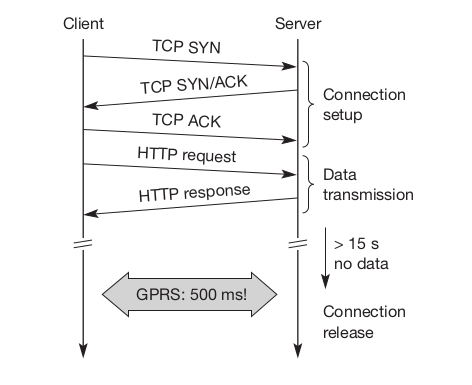
\includegraphics[width=0.8\textwidth]{tcp-connection-setup-overhead}
	\caption{Example TCP connection setup overhead}\label{fig:tcp_connection_setup_overhead}
\end{figure}


This led to the development of a transaction-oriented TCP (T/TCP). 
\begin{itemize}
	\item T/TCP can combine packets for connection establishment and connection release with user data packets. 
	\item This can reduce the number of packets down to two instead of seven.
\end{itemize}

\subsubsection{Advantages}
\paragraph*{Overhead Reduction}
The obvious advantage for certain applications is the reduction in the overhead which standard TCP has for connection setup and connection release. 

\subsubsection{Disadvantages}
\paragraph*{Requires Changes in MH and all CH}
T/TCP is not the original TCP anymore, so it requires changes in the mobile host and all correspondent hosts, which is a major disadvantage. 

\paragraph*{Mobility No Longer Transparent}
This solution no longer hides mobility. 

\paragraph*{Exhibits Several Security Problems}
Furthermore, T/TCP exhibits several security problems.


%%%%%%%%%%%%%%%%%%%%%%%%%%%%%
%							%
%		TABLE				%
%							%
%%%%%%%%%%%%%%%%%%%%%%%%%%%%%
\begin{landscape}
	\section[Classical Enhancements to TCP]{Overview of Classical Enhancements to TCP for Mobility}
	
\begin{longtable}[ht!]{@{}>{\raggedright\arraybackslash}p{3cm}>{\raggedright\arraybackslash}p{4.1cm}>{\raggedright\arraybackslash}p{4.1cm}>{\raggedright\arraybackslash}p{4.1cm}@{}}
	\caption{Overview of classical enhancements to TCP for mobility.}{\label{tab:classical_enhancments_tcp}} \\
	
	\toprule
	\textbf{Approach} & \textbf{Mechanism} & \textbf{Advantages} & \textbf{Disadvantages}\\
	\midrule
	
	\endfirsthead
	\multicolumn{2}{c}%
	{\tablename\ \thetable\ -- \textit{Continued from previous page}} \\
	
	\hline
	\textbf{Approach} & \textbf{Mechanism} & \textbf{Advantages} & \textbf{Disadvantages}\\
	\hline
	\endhead \hline
	\multicolumn{4}{r}{\textit{Continued on next page $\ldots$}} \\
	\endfoot
	\endlastfoot
	
	\textbf{Indirect TCP} & Splits TCP connection into two connections & Isolation of wireless link, simple & Loss of TCP semantics, higher latency at handover, security problems \tabularnewline
	
	\textbf{Snooping TCP} & Snoops data and acknowledgements, local retransmission & Transparent for end-to-end connection, MAC integration possible & Insufficient isolation of wireless link, security problems \tabularnewline
	

	\textbf{M-TCP} & Splits TCP connection, chokes sender via window size & Maintains end-to-end semantics, handles long term and frequent disconnections & Bad isolation of
	wireless link, processing overhead due to bandwidth management, security problems \tabularnewline


	\textbf{Fast retransmit/fast revcovery} & Avoids slow-start after roaming & Simple and
	efficient & Mixed layers, not transparent \tabularnewline


	\textbf{Transmission/time-out freezing} & Freezes TCP state at disconnection, resumes after reconnection & Independent of content, works for longer interruptions & Changes in TCP required, MAC dependent \tabularnewline

	\textbf{Selective retransmission} & Retransmits only lost data & Very effficient & Slightly more complex receiver software, more buffer space needed \tabularnewline


	\textbf{Transaction oriented TCP} & Combines connection setup/release and data transmission & Efficient for certain applications & Changes in TCP required,
	not transparent, security problems \tabularnewline
		
	\bottomrule
	
\end{longtable}
\end{landscape}
%
%
%Table \ref{tab:classical_enhancments_tcp} shows an overview of the classical mechanisms presented together with some advantages and disadvantages. The approaches are not all exclusive, but can be combined. Selective re-transmission, for example, can be used
%together with the others and can even be applied to fixed networks.
%
%An additional scheme that can be used to reduce TCP overhead is header
%compression. Using tunneling schemes as in mobile IP together with TCP, results in protocol headers of 60 byte in case of
%IPv4 and 100 byte for IPv6 due to the larger addresses. Many fields in the IP and
%TCP header remain unchanged for every packet. Only just transmitting the differences is often sufficient. Especially delay sensitive applications like, e.g.,
%interactive games, which have small packets benefit from small headers.
%However, header compression experiences difficulties when error rates are high
%due to the loss of the common context between sender and receiver.
%
%With the new possibilities of wireless wide area networks (WWAN) and their
%tremendous success, the focus of research has shifted more and more towards
%these 2.5G/3G networks. Up to now there are no final solutions to the problems
%arising when TCP is used in WWANs. However, some guidelines do exist.
%

\section{TCP over 2.5G/3G Wireless Networks}
The TCP over 2.5G/3G wireless networks describes a profile for optimizing TCP over wireless \gls{wan}s such as \gls{gsm}, \gls{gprs}, \gls{umts}. The focus on 2.5G/3G for transport of internet data is important as already billions of people use mobile phones and it is obvious that the mobile phone systems will also be used to transport arbitrary internet data.

\subsection[Characteristics]{Characteristics to be Considered}{\label{sec:characteristics_2_3_g}}
The following characteristics have to be considered when deploying applications over 2.5G/3G wireless links:

\subsubsection{Data Rates}
Typically, data rates are asymmetric as it is expected that users will download more data compared to uploading. Uploading is limited by the limited battery power. In cellular networks, asymmetry does not exceed 3–6 times, however, considering broadcast systems as additional distribution media (digital radio, satellite systems), asymmetry may reach a factor of 1,000.

\subsubsection{Latency}
All wireless systems comprise elaborated algorithms for error correction and protection, such as \gls{fec}, checksumming, and interleaving. FEC and interleaving let the \gls{rtt} grow to several hundred milliseconds up to some seconds.


\subsubsection{Jitter}
Wireless systems suffer from large delay variations or \textit{delay spikes}. Reasons for sudden increase in the latency are: 
\begin{itemize}
	\item link outages due to temporal loss of radio coverage,
	\item blocking due to high-priority traffic, or handovers
\end{itemize}

Handovers are quite often only virtually seamless with outages reaching from some $ 10 ms $ to several seconds.

\subsubsection{Packet Loss}
Packets might be lost during handovers or due to corruption. Due to link-level re-transmissions the loss rates of 2.5G/3G systems due to corruption are relatively low (but still orders of magnitude higher than, e.\ g.\, fiber connections). However, recovery at the link layer appears as \textit{jitter} to the higher layers.


\subsection[Configuration Parameters]{Configuration Parameters to Adapt TCP to Wireless Environments}

Based on the characteristics (see Section \ref{sec:characteristics_2_3_g}), configuration parameters to adapt TCP to wireless environments are:

\subsubsection{Large Windows}
TCP should support large enough window sizes based on the bandwidth delay experienced in wireless systems. With the help of the windows scale option and larger buffer sizes this can be accomplished. A larger initial window segments may increase performance particularly for short transmissions.


\subsubsection{Limited Transit}
This mechanism is an extension of Fast Re-transmission/Fast Recovery and is particularly useful when small amounts of data are to be transmitted (standard for, e.\ g.\, web service requests).

\subsubsection{Large MTU}
The larger the MTU (Maximum Transfer Unit) the faster TCP increases the congestion window. Large MTUs may be used to increase performance. MTU path discovery should be used to employ larger segment sizes instead of assuming the small default MTU.


\subsubsection[Selective Acknowledgment]{Selective Acknowledgment (SACK)}
SACK allows the selective re-transmission of packets and is almost always beneficial compared to the standard cumulative scheme.


\subsubsection[Explicit Congestion Notification]{Explicit Congestion Notification (ECN)}
ECN allows a receiver to inform a sender of congestion in the network by setting the ECN-Echo flag on receiving an IP packet that has experienced congestion. This mechanism makes it easier to distinguish packet loss due to transmission errors from packet loss due to congestion.


\subsubsection{Timestamp}
With the help of timestamps higher delay spikes can be tolerated by TCP without experiencing a spurious timeout. The effect of bandwidth oscillation is also reduced.

\subsubsection{No Header Compression}
Header compression is not compatible with TCP options such as SACK or timestamps.

